\documentclass[11pt]{article}
\usepackage{amsmath}
\usepackage{geometry}                % See geometry.pdf to learn the layout options. There are lots.
\geometry{letterpaper}                   % ... or a4paper or a5paper or ... 
%\geometry{landscape}                % Activate for for rotated page geometry
%\usepackage[parfill]{parskip}    % Activate to begin paragraphs with an empty line rather than an indent
\usepackage{graphicx}
\usepackage{amssymb}
\usepackage{epstopdf}
\DeclareGraphicsRule{.tif}{png}{.png}{`convert #1 `dirname #1`/`basename #1 .tif`.png}

%Don't list section numbers
\setcounter{secnumdepth}{0}

\title{CS 1653: Applied Cryptography and Network Security\\Term Project, Phase 3}
\author{Lindsey ``Hellman" Bieda\quad\texttt{leb35@pitt.edu}\qquad Tucker ``Diffie" Trainor\quad\texttt{tmt33@pitt.edu}}
\date{March 2, 2012} % Activate to display a given date or no date

\begin{document}
\maketitle
\section{Introduction: Cryptographic Techniques}
Protecting communication over networks is a byzantine affair involving prime numbers, modulo arithmetic, and inscrutable cipher text. No one protocol is enough to cover all vulnerabilities of a secure file server implementation, and often hybridization of protocols is the best solution to thorny security issues. In our implementation of a secure file server, we will include proven methods from both private key cryptography and public key cryptography, and sometimes even combine the two. From the realm of private key cryptography, we will use AES for block cipher encryption. From public key cryptography, we use RSA public/private key encryption to leverage security and efficiency where possible. We will also implement hash functions such as SHA-1 for authenticating data where necessary.
% Threat 1
\section{Threat 1: Unauthorized Token Issuance}
\subsection{Threat Description}
For a user to begin using the secure file server, they must be issued a token with which they can perform all the functions of the Group and File Servers. Thus, we need to protect each user's token from anyone other than the user. In Phase 2 of the project, we considered the users trustworthy and therefore didn't require any credentials other than knowing the username of the token's owner. This is almost completely insecure against any malicious agent who knows a username on the system, as they can simply enter any valid username to be issued that user's token.
\subsection{Mechanism Description}
We can implement a password mechanism to verify that a user is who they claim to be. By requiring a login sequence consisting of a username and password tuple, we can do a basic authentication of the user. Before defining a sequence of operations to authorize issuance of a token, we must list assumptions of existing conditions:
\begin{itemize}
\item{}The user has been created by an administrator and is in possession of their correct password.
\item{}The user has connected through the client application to the Group Server and has already saved the Group Server's public key in the file that their client uses to store public keys.
\item{}The Group Server's private key has not been compromised.
\item{}The user has an active connection to the Group Server.
\end{itemize}
\begin{figure}[htbp]
\begin{center}
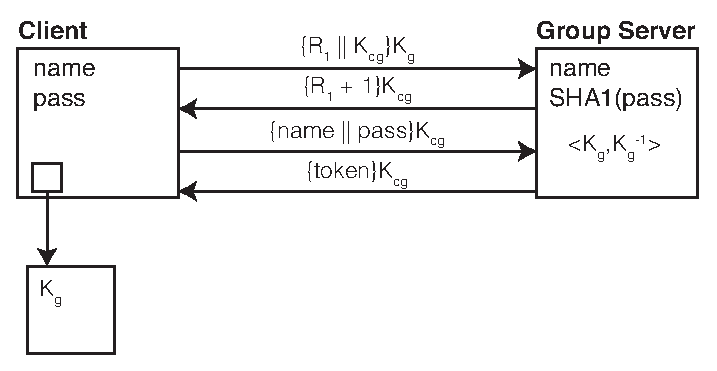
\includegraphics{threat1.eps}
\caption{Threat 1 Mechanism}
\label{threat1}
\end{center}
\end{figure}
With these assumptions in place, we can outline the steps to maintain the confidentiality and integrity of each user's token:
\begin{enumerate}
\item{}Authenticate the Group Server -- through the client, the users generates a random number R$_1$ and concatenate it with a randomly chosen AES key K$_{\text{cg}}$. This data is then encrypted with the Group Server's public key K$_\text{g}$ via RSA, all represented as \{R$_1||$K$_{\text{cg}}$\}K$_\text{g}$. The Group Server. The Group Server decrypts this cipher using its private key K$_\text{g}^{-1}$. The Group Server now uses the shared symmetric key K$_{\text{cg}}$ to encrypt the value of R$_1$+1, represented as \{R$_1$+1\}K$_{\text{cg}}$, and sends this new cipher to the client. The client decrypts the cipher, and by noting that the value R$_1$ and the key K$_\text{cg}$ was successfully decrypted by the Group Server, the client has authenticated the Group Server.
\item{}Authenticate the user -- Now that  the shared symmetric key K$_\text{cg}$ is agreed upon, the user encrypts their name and password with it, represented as \{name$||$pass\}K$_\text{cg}$, as sends the cipher text to the Group Server. The Group Server decrypts the cipher text to recover the user's name and password, and then performs an SHA-1 message digest on the password. As the Group Server stores the hashes of passwords instead of the passwords themselves, it checks the SHA-1 hash of the user-submitted password against what it has stored. If the two hash values agree, the user is authenticated to the Group Server.
\item{}Issue token -- The Group Server can now send the user their token over the encrypted channel, ensuring that only the user, who is authorized to receive the token, is able to access it.
\end{enumerate}
We store the username with a hash of the password instead of the password in cleartext to avoid revealing passwords in the event of a compromise to the Group Server, where a hash table of usernames and hashes would be stored. The user would enter their password, which would be sent to the Group Server over an encrypted channel. If the hashes match, the user is authenticated as who they claim to be and issued their token, otherwise access is denied.
\subsection{Correctness and Security of Mechanism}
To maintain correctness, both parties will need to agree on the shared symmetric key K$_\text{cg}$ for encryption and decryption to be possible. They must also agree on the protocol of accepting the random number challenge R$_1$ and adding to it as a response. Security is maintained by the use of public key cryptography to encrypt the initial exchanges that establish authentication and generate a shared secret key, and then symmetric key cryptography to encrypt all further exchanges between the two parties using the shared secret key.
% Threat 2
\section{Threat 2: Token Modification/Forgery}
\subsection{Threat Description}
By modifying or forging tokens issued by the Group Server, a user may be able to gain access to files that would otherwise be forbidden. By changing the group information embedded in a token, a malicious user can access groups that they are not members of, which would grant unauthorized access to files belonging to those groups. Furthermore, if a malicious user assigns him or herself as the owner of a specific group, he or she will have the ability to add or delete group members, as well as freely modify files belonging to that group. This threat is a direct attack on the integrity of a secure group server.
\subsection{Mechanism Description}
In order to maintain the integrity of token issuance, we should verify that a token is valid every time an operation involving a token is invoked on a File Server. In order to efficiently carry out this operation, which may occur frequently during peak server activity, we can modify the Token class so that it both stores a digital signature signed by the Group Server in addition to a method that allows the File Server (or any third party) to perform a check on the token. By tokenizing the contents of a Token object into a string, the Group Server can use its private key K$_\text{g}^{-1}$ to sign the string. Any third party who wishes to verify a token can call upon the method that creates the tokenized string and can compare it to the digital signature, which can be decrypted with the Group Server's public key K$_\text{g}$. We make the following assumptions in this mechanism:
\begin{itemize}
\item{}The third party has access to the Group Server's public key.
\item{}The third party has access to the Token class methods in order to extract the contents of the user's token.
\item{}The Group Server's private key has not been compromised.
\end{itemize}
\begin{figure}[htbp]
\begin{center}
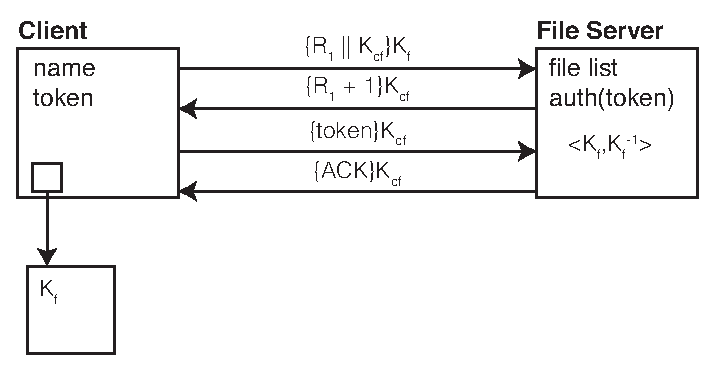
\includegraphics{threat2.eps}
\caption{Threat 2 Mechanism}
\label{threat2}
\end{center}
\end{figure}
With these assumptions in place, we can begin the protocol to verify a user's token:
\begin{enumerate}
\item{}Perform an exchange to establish a shared symmetric key so that the two parties can communicate securely. (see Threat 1 for expanded explanation)
\item{}The user sends their token to the third party (e.g. a File Server) using the secret key to encrypt it.
\item{}The third party decrypts the token, retrieves its tokenized string and its digital signature. After decrypting the signature with K$_\text{g}$, it compares the two strings.
\item{}If the two strings match, the third party returns an acknowledgement. If forgery is suspected, the third party may terminate the connection or take other evasive action.
\end{enumerate}
\subsection{Correctness and Security of Mechanism}
Correctness is partly dependent on the Group Server and how it signs tokens. As long as the integrity of these signatures is ensured, then the only other factor for correctness is the comparison of the decrypted signature and what is provided by the token's own method. Security is held by the secrecy of the Group Server's private key, which we assume is safe from attack, and by the strength of the encryption of the communication channel between the two parties.
% Threat 3
\section{Threat 3: Unauthorized File Servers}
\subsection{Threat Description}
The purpose of a secure file server is that, put simply, your files are secure. If a user can unknowingly be directed to an unauthorized file server, any other security safeguards are rendered moot, thus threatening the confidentiality of the user's files and the perceived integrity of the entire service. If a user can be convinced that they are connected to file server $f$ while actually being connected to a malicious file server $f^\prime$, they are at risk of uploading confidential data to an untrusted source or downloading malicious content from an untrusted source.
\subsection{Mechanism Description}
In order for a file server to be trusted by a user, it must provide some authentication to the user that only the actual server can know. Though certificates would be an ideal solution, they are outside the scope of our project. Instead, we can rely on public and private key pairs as a way of validating a File Server. Upon the first connection to a File Server $f$, the user will be asked if they wish to accept the public key K$_\text{f}$. If the user agrees, K$_\text{f}$ is stored by the user through their client application along with other identifying details of the File Server (e.g. server name, IP address, etc.). When the user wishes to authenticate the server, he or she can use K$_\text{f}$ to encrypt a challenge to $f$. If $f$ is in possession of the private key K$_\text{f}^{-1}$, then $f$ is able to return the challenge to the user and authentication is complete. An unauthorized server $f^\prime$ would be unable to correctly guess K$_\text{f}^{-1}$ and therefore could not correctly decrypt of the challenge and complete authentication. We make the following assumptions in this mechanism:
\begin{itemize}
\item{}The initial contact between the user and $f$ was legitimate and the user was able to correctly store $f$'s information and public key.
\item{}The private key of $f$ has not been compromised.
\end{itemize}
\begin{figure}[htbp]
\begin{center}
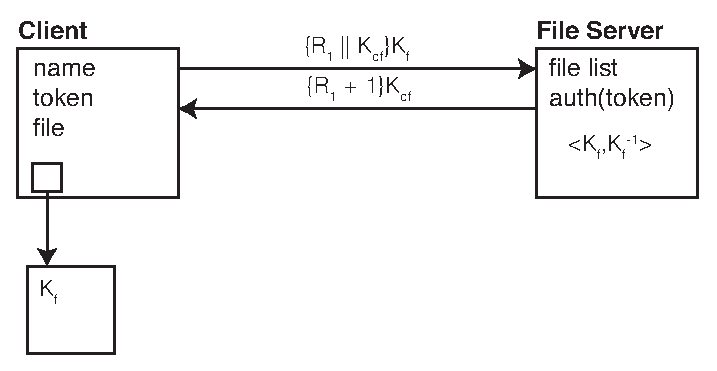
\includegraphics{threat3.eps}
\caption{Threat 3 Mechanism}
\label{threat3}
\end{center}
\end{figure}
With these assumptions in place, we can begin the protocol to authenticate a File Server:
\begin{enumerate}
\item{}Begin an exchange to establish a shared symmetric key so that the two parties can communicate securely. (see Threat 1 for expanded explanation)
\item{}If the File Server is able to decrypt the message with its private key, then it can only be the server with which the user wishes to communicate with. The File Server returns the challenge value R$_1$ incremented by 1 and encrypts this value with the agreed upon shared symmetric key.
\item{}The user decrypts the returned challenge and sees that the challenge was correctly interpreted, and thus the File Server is authenticated to the user.
\end{enumerate}
\subsection{Correctness and Security of Mechanism}
Security is held by the secrecy of the File Server's private key, which we assume is safe from attack, and by the strength of the encryption of the communication channel between the two parties. Correctness is held when the user and the File Server agree on the challenge protocol and how the File Server should increment the challenge value.
% Threat 4
\section{Threat 4: Information Leakage via Passive Monitoring}
\subsection{Threat Description}
Suppose Eve can listen to an information exchange between Alice and Bob. Even without being able to interrupt or modify the exchange, Eve can still glean enough information to perform malicious acts. If insufficient security is in place, Eve may be able to gather enough data to
\begin{itemize}
\item know the contents of the exchanges;
\item to impersonate Alice or Bob;
\item use offline password guessing to discover passwords or other secret information.
\end{itemize}
Eve does not need to be an active participant in a conversation to illicitly benefit from it, and thus exchanges between Alice and Bob must be kept secure. Or, to put into context of a secure file server, any exchanges between a user and any server (or even between servers) must be kept confidential if proper security is to be maintained.
\subsection{Mechanism Description}
To maintain a secure channel between Alice and Bob during a continuous series of messages, the most efficient solution may be to create a session key between them. A session key avoids having to recreate a secure channel after each exchange, resulting in increased efficiency over alternative methods that would require more frequent overhead or computation. To create a session key, we can implement public-key authentication protocols to provide authentication between two parties and provide them with a shared secret key. The secret key can then be used as a password for symmetric key encryption of all communication during the lifetime of the session. The steps to follow are similar to Threat 1 and Threat 3, in which both parties have public/private key pairs. Similar assumptions can be made in this case as well:
\begin{itemize}
\item{}Alice and Bob have access to each other's private keys, and are assured that they are indeed correct.
\item{}Neither party's private keys have been compromised.
\end{itemize}
\subsection{Correctness and Security of Mechanism}
If the key exchange is performed securely, then each session is properly encrypted. Correctness can be maintained in following the symmetric key exchange protocols and proper order of public/private key encryption. Security is maintained in the strength of the passwords and encryption methods.
\section{Summary and Errata}
There are common elements to the protocols that address the above threats. Since Threat 4 involves eavesdropping, most if not all communication over the network will need to be encrypted. Thus, handshake and/or authentication protocols will be present in many of the implementations we have discussed. Implementation may show that similar code can be easily adapted to each different threat as a basis of establishing a secure communication channel.

There was a lot of excited chatter by one of the group members in regards to Diffie-Hellman key exchanges as a starting point to establishing shared symmetric keys. In practice, this is not efficient nor really necessary, as RSA key pairs are used by all endpoints of communication in our secure file server model. With these keys already in place, creating temporary public keys is a waste of time. With this in mind, the Diffie-Hellman fanatic has been admonished not to reinvent the fifth wheel.
\end{document}
